\section{Full result graphs}
\label{sec:appendix-graphs}

Figure~\ref{fig:scatter-full-2x4} shows the full 8-coefficient scatter
for the 2x4 setup: each subplot is a scatter of $300$ test samples
with the identity reference line and the Pearson correlation between
predicted and true coefficients. The Pearson $r$ values range from
roughly $0.92$ to $0.96$ across the eight coefficients.

\begin{figure}[H]
  \centering
  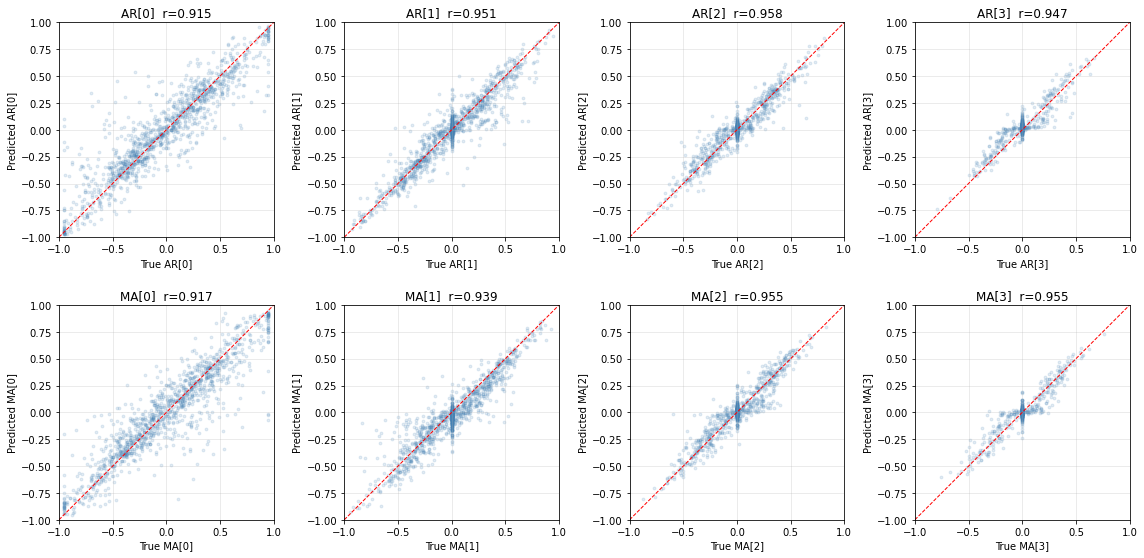
\includegraphics[width=\linewidth]{figures/recovery_scatter_full_2x4.png}
  \caption{Full 8-coefficient scatter for the 2x4 (ARMA(4, 4))
    configuration: AR$_0$ to AR$_3$ on the top row, MA$_0$ to MA$_3$
    on the bottom row.}
  \label{fig:scatter-full-2x4}
\end{figure}

Figure~\ref{fig:scatter-full-2x2} shows the equivalent 4-coefficient
scatter for the 2x2 setup. The Pearson $r$ values range from $0.94$
to $0.97$, slightly higher than for the 2x4 case, consistent with the
higher overall recovery ratio of $8.34$.

\begin{figure}[H]
  \centering
  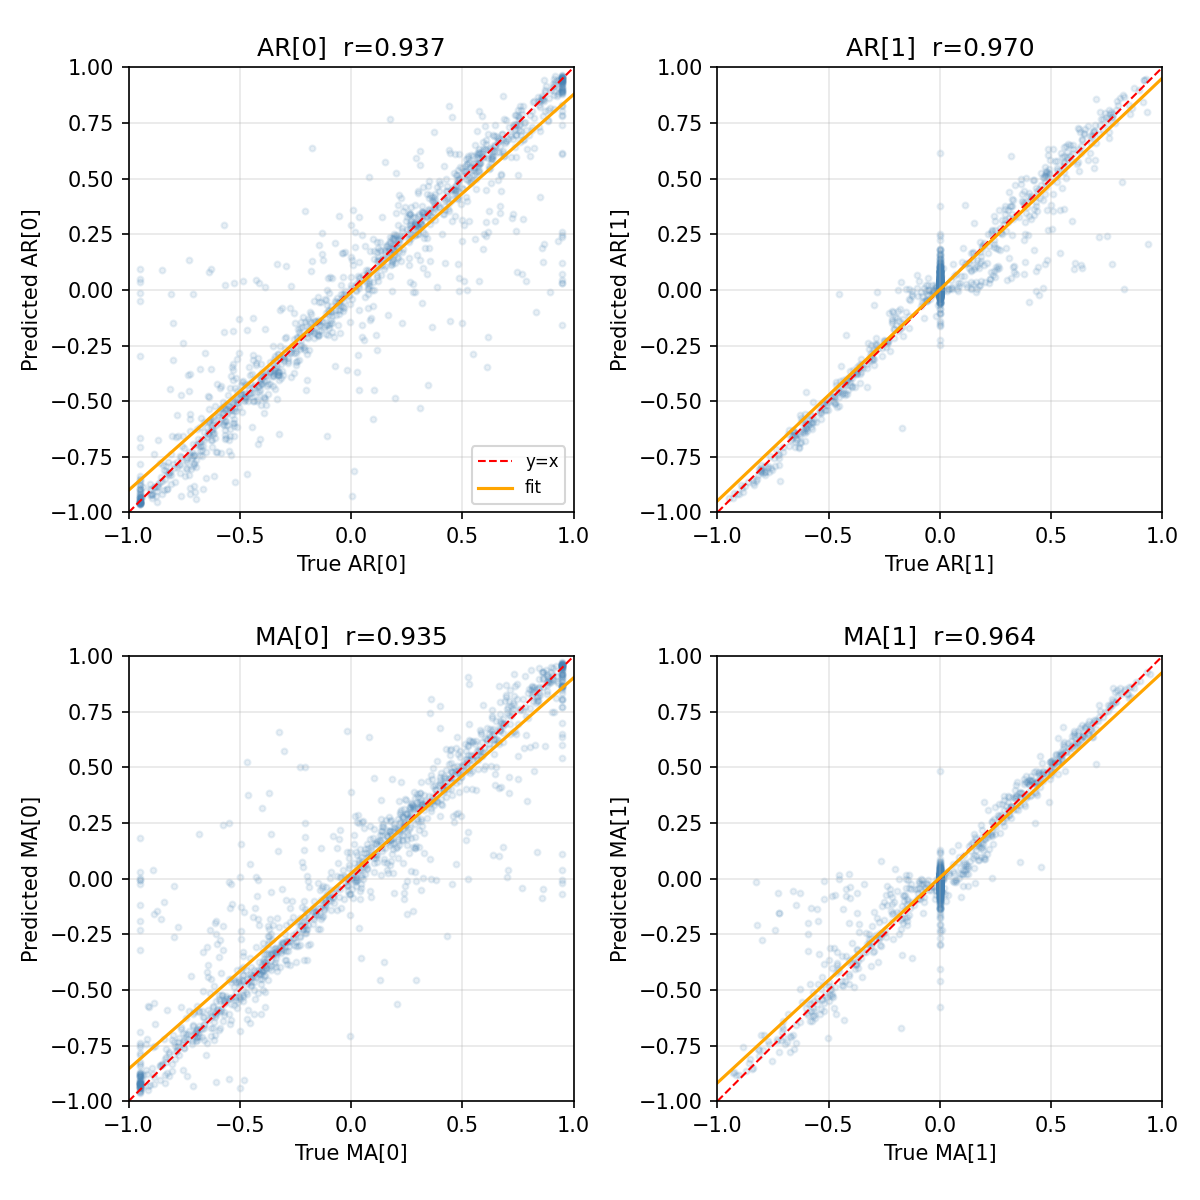
\includegraphics[width=0.6\linewidth]{figures/recovery_scatter_full_2x2.png}
  \caption{Full 4-coefficient scatter for the 2x2 (ARMA(2, 2))
    configuration: AR$_0$ and AR$_1$ on the top row, MA$_0$ and MA$_1$
    on the bottom row.}
  \label{fig:scatter-full-2x2}
\end{figure}

Figure~\ref{fig:error-dist-2x4} shows the per-sample MSE distribution
for the 2x4 head on $200$ test samples.

\begin{figure}[H]
  \centering
  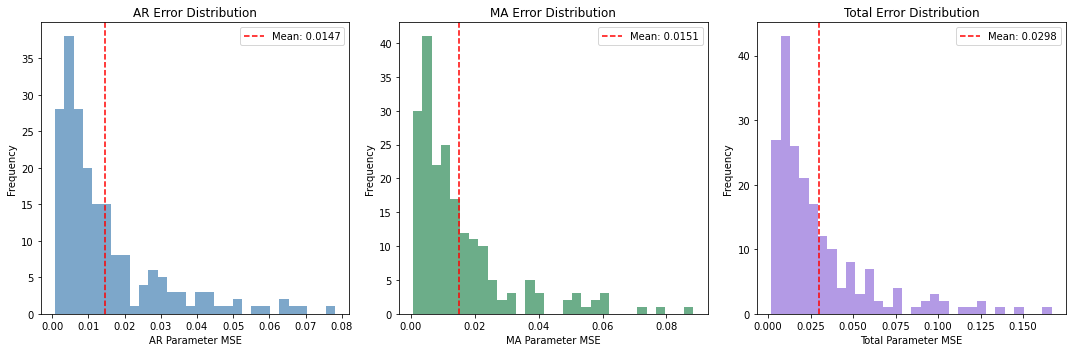
\includegraphics[width=0.7\linewidth]{figures/recovery_error_distributions.png}
  \caption{Per-sample MSE distributions for the recovery head on the
    2x4 configuration.}
  \label{fig:error-dist-2x4}
\end{figure}
